\chapter[Datos]{Datos}
\label{Chap3}

Para este proyecto disponemos de los siguientes datos obtenidos de distintas páginas web:
\begin{itemize}
	\item Nivel (m)
	\item Caudal ($m^3/s$)
	\item Precipitación (mm)
	\item Temperatura (ºC)
	\item Humedad (\%)
	\item Radiación ($W/m^2$)
\end{itemize}
A su vez, dispondremos de la fecha y hora en la que se hicieron la lectura de los datos, junto con los códigos y coordenadas de las estaciones sobre las cuales obtenemos los datos.

\section{Aemet}
La Agencia Estatal de Meteorología (AEMET) es el Servicio Meteorológico Nacional y Autoridad Meteorológica del Estado, siendo su objetivo es la monitorización y predicción de fenómenos meteorológicos.
\newline
\newline
AEMET dispone de una API de obtención de datos llamada AEMET OpenData la cual no usaremos pues muchos de los datos que se obtienen de esta manera no nos son útiles.
\newline
\newline
Como se ve en la imagen \ref{fig:ej3}, dentro de la web podemos encontrar de forma accesible múltiples datos relacionados con la meteorología tomados cada hora, de los cuales seleccionaremos únicamente temperatura, precipitación y humedad, puesto que los datos relacionados con el viento o la presión atmosférica no son tan relevantes para este proyecto.

\begin{figure} [h!]
	\centering
	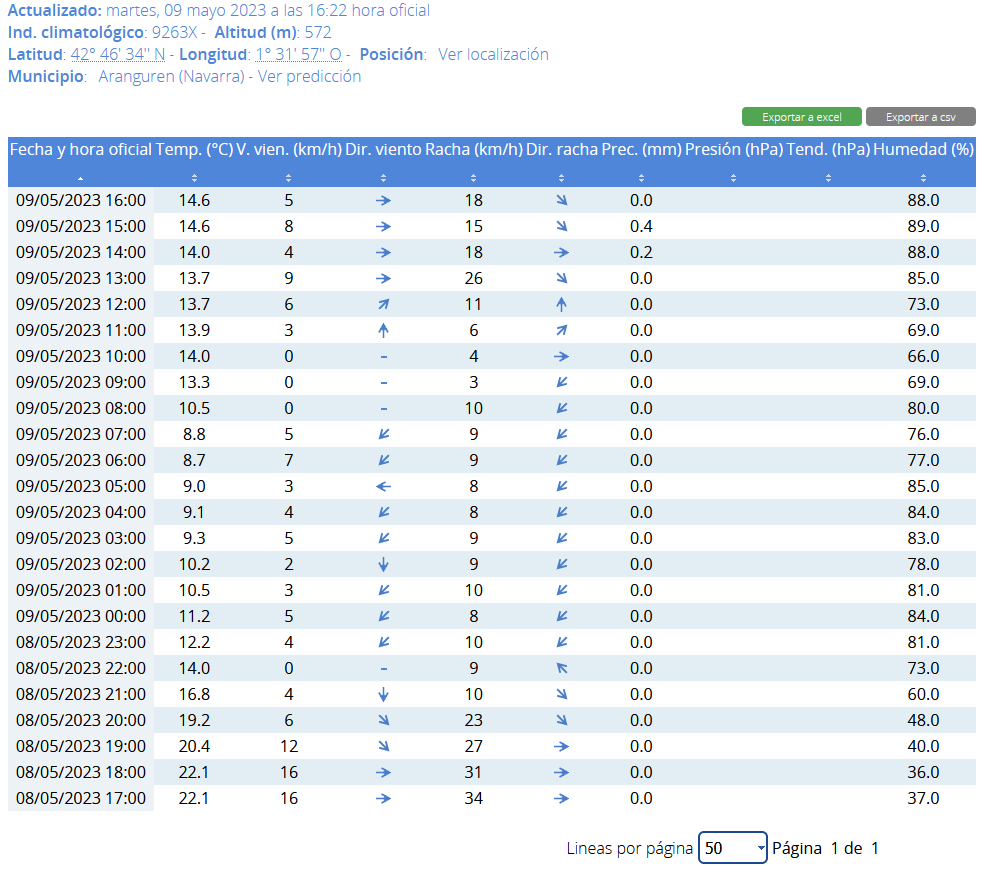
\includegraphics[width=0.7\textwidth]{fig/Aemet.png}
	\caption[Página Aemet de la estación en Aranguren (Navarra)]{Página Aemet}
	\label{fig:ej3}
\end{figure}

\section{El Agua en Navarra}
En esta página encontraremos los datos tanto del nivel de los ríos como de su caudal en los últimos 15 días en periodos de 10 minutos, siendo una de las fuentes principales de datos.
\newline
\newline
La sección de aforos en la página \ref{fig:ej4} muestra un mapa de Navarra y esta estructurada en 6 regiones, Norte, Arga, Ega, Ebro alto, Ebro bajo y Aragón, accediendo a cada región nos aparece el mapa de la región dándonos acceso a todas las estaciones en la zona.
\newline
\newline
Una vez dentro de la estación tendremos la posibilidad de observar los datos, primeramente en forma de gráfica y en caso de quererlo en forma numérica, pero no se puede acceder a los datos numéricos sin antes haber visitado la versión gráfica \ref{fig:ej5}.
\newline
\newline
Debido a este problema, para la obtención de los datos primero cargamos la web gráfica y le pasamos un script JavaScript para pulsar el botón que finalmente nos da acceso a los datos deseados.

\begin{figure} [h!]
	\centering
	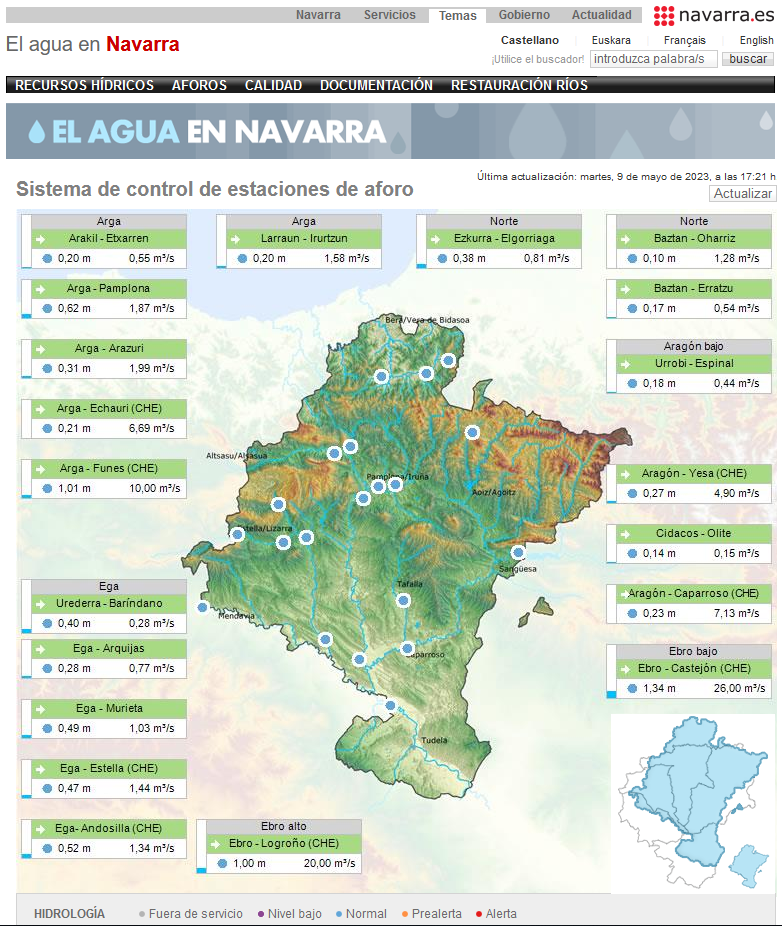
\includegraphics[width=0.7\textwidth]{fig/AguaEnNavarra.png}
	\caption[Página principal de aforos de El Agua en Navarra]{Página El Agua en Navarra}
	\label{fig:ej4}
\end{figure}

\begin{figure} [h!]
	\centering
	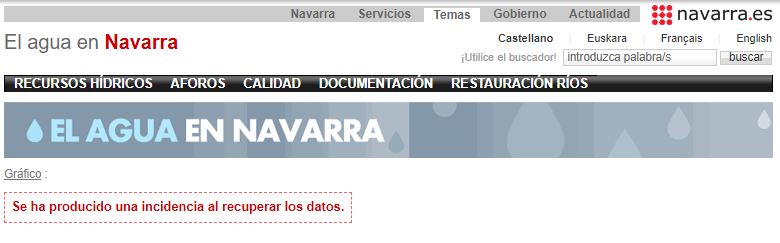
\includegraphics[width=0.7\textwidth]{fig/ErrorAguaEnNavarra.png}
	\caption[Página principal de aforos de El Agua en Navarra]{Página El Agua en Navarra}
	\label{fig:ej5}
\end{figure}